\chapter{Поверхности второго порядка}

$$ a_{11}x^2 + 2a_{12}xy + a_{22}y^2 + 2a_{23}yz + a_{13}xz + a_{33}^2 + 2b_1x + 2b_2y + 2b_3z + b_4 = 0 $$

\begin{algorithm}
    \hfill
    \begin{enumerate}
        \item Поворотом избавляемся от $a_{12}, a_{13}, a_{23}$ (докажем позже)
        \item Сдвиги:
        \begin{itemize}
            \item Если $a_{11} \ne 0$, то считаем, что $b_1 = 0$ \\
            ......
            \item Если $a_{11} = 0$ и $b_1 \ne 0$, то считаем $b_4 = 0$ \\
            ......
            \item Тут разные типы:
            \begin{enumerate}
                \item Эллиптический ($a_{11} > 0$, $a_{22} > 0$, $a_{33} > 0$)
                $$ a_{11}x^2 + a_{22}y^2 + a_{33}z^2 + b_4 = 0 $$
                \begin{enumerate}
                    \item $b_4 < 0$
                    $$ \frac{x^2}{a^2} + \frac{y^2}{b^2} + \frac{z^2}{c^2} = 1 \text{ -- эллипсоид} $$
                    \item $b_4 = 0$
                    $$ \frac{x^2}{a^2} + \frac{y^2}{b^2} + \frac{z^2}{c^2} = 0 \text{ -- точка} $$
                    \item $b_4 > 0$
                    $$ \frac{x^2}{a^2} + \frac{y^2}{b^2} + \frac{z^2}{c^2} = -1 \text{ -- мнимый эллипсоид} $$
                \end{enumerate}
                \item Гиперболический ($a_{11}, a_{12} > 0$, $a_{33} < 0$) (рис. \ref{im:1}) \\
                Тоже 3 случая, в зависимости от знака $b_4$:
                \begin{enumerate}
                    \item $ \frac{x^2}{a^2} + \frac{y^2}{b^2} - \frac{z^2}{c^2} = 1 $ -- однополостный гиперболоид
                    \item $ \frac{x^2}{a^2} + \frac{y^2}{b^2} - \frac{z^2}{c^2} = 0 $ -- конус
                    \item $ \frac{x^2}{a^2} + \frac{y^2}{b^2} - \frac{z^2}{c^2} = -1 $ -- двухполостный гиперболоид
                \end{enumerate}
                \item Параболический ($a_{33} = 0$) (рис. \ref{im:2})
                \begin{enumerate}
                    \item $b_3 \ne 0$, $a_{11}, a_{22} \ne 0$ ($\implies b_4 = 0$)
                    $$ a_{11}x^2 + a_{22}y^2 + 2b_3z = 0 $$
                    \begin{enumerate}
                        \item $\frac{x^2}{a^2} + \frac{y^2}{b^2} = 2z $ -- эллиптический параболоид
                        \item $\frac{x^2}{a^2} + \frac{y^2}{b^2} = 2z $ -- гиперболический параболоид
                    \end{enumerate}
                    \item $b_3 = 0$. Нет зависимости от $z$
                    \begin{enumerate}
                        \item $\frac{x^2}{a^2} + \frac{y^2}{b^2} = 1$ -- эллиптический цилиндр
                        \item $\frac{x^2}{a^2} + \frac{y^2}{b^2} = 0$ -- прямая
                        \item $\frac{x^2}{a^2} + \frac{y^2}{b^2} = -1$ -- тоже прямая
                        \item $\frac{x^2}{a^2} - \frac{y^2}{b^2} = 1$ -- гиперболический цилиндр
                        \item $\frac{x^2}{a^2} - \frac{y^2}{b^2} = 0$ -- пара пересекающихся плоскостей
                        \item $y^2 = 2px$ -- параболический цилиндр
                        \item $\frac{x^2}{a^2} = 1$ -- пара параллельных плоскостей
                        \item $\frac{x^2}{a^2} = 0$ -- плоскость
                        \item $\frac{x^2}{a^2} = -1$ -- $\O$
                    \end{enumerate}
                \end{enumerate}
            \end{enumerate}
        \end{itemize}
    \end{enumerate}
\end{algorithm}

\begin{figure}[!ht]
    \begin{subfigure}{0.45\textwidth}
    	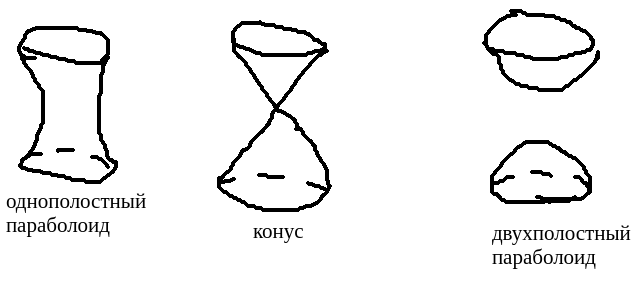
\includegraphics[scale=0.4]{giperb}
        \caption{Гиперболический тип}
        \label{im:1}
    \end{subfigure}
    \begin{subfigure}{0.45\textwidth}
    	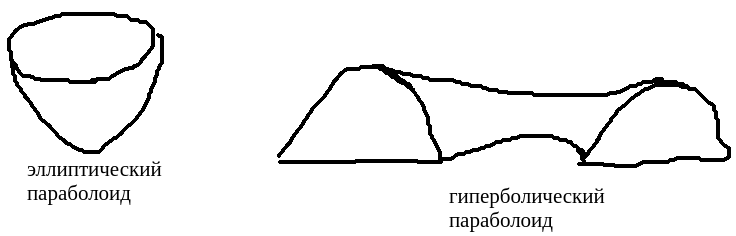
\includegraphics[scale=0.4]{parab}
        \caption{Параболический тип}
        \label{im:2}
    \end{subfigure}
    \caption{Классификация}
\end{figure}
